\documentclass[]{scrartcl}
\usepackage{lmodern}
\usepackage{amssymb,amsmath}
\usepackage{ifxetex,ifluatex}
\usepackage{fixltx2e} % provides \textsubscript
\ifnum 0\ifxetex 1\fi\ifluatex 1\fi=0 % if pdftex
  \usepackage[T1]{fontenc}
  \usepackage[utf8]{inputenc}
\else % if luatex or xelatex
  \ifxetex
    \usepackage{mathspec}
  \else
    \usepackage{fontspec}
  \fi
  \defaultfontfeatures{Ligatures=TeX,Scale=MatchLowercase}
\fi
% use upquote if available, for straight quotes in verbatim environments
\IfFileExists{upquote.sty}{\usepackage{upquote}}{}
% use microtype if available
\IfFileExists{microtype.sty}{%
\usepackage{microtype}
\UseMicrotypeSet[protrusion]{basicmath} % disable protrusion for tt fonts
}{}
\usepackage{hyperref}
\hypersetup{unicode=true,
            pdftitle={Angabe},
            pdfauthor={Team\ldots{}},
            pdfborder={0 0 0},
            breaklinks=true}
\urlstyle{same}  % don't use monospace font for urls
\IfFileExists{parskip.sty}{%
\usepackage{parskip}
}{% else
\setlength{\parindent}{0pt}
\setlength{\parskip}{6pt plus 2pt minus 1pt}
}
\setlength{\emergencystretch}{3em}  % prevent overfull lines
\providecommand{\tightlist}{%
  \setlength{\itemsep}{0pt}\setlength{\parskip}{0pt}}
\setcounter{secnumdepth}{5}
% Redefines (sub)paragraphs to behave more like sections
\ifx\paragraph\undefined\else
\let\oldparagraph\paragraph
\renewcommand{\paragraph}[1]{\oldparagraph{#1}\mbox{}}
\fi
\ifx\subparagraph\undefined\else
\let\oldsubparagraph\subparagraph
\renewcommand{\subparagraph}[1]{\oldsubparagraph{#1}\mbox{}}
\fi

\usepackage{graphicx}
\usepackage{array}
\usepackage{ragged2e}
\usepackage[section]{placeins}
\makeatletter
\AtBeginDocument{%
  \expandafter\renewcommand\expandafter\subsection\expandafter{%
    \expandafter\@fb@secFB\subsection
  }%
}
\makeatother
 
\title{Angabe 1}
\providecommand{\subtitle}[1]{}
\subtitle{Untertitel}
\author{Daniel Graf, Dimitrie Diez, Arne Schöntag, Peter Müller}
\date{}

\begin{document}
\maketitle


\tableofcontents

\section{Einführung}
Da heutzutage das Laufverhalten von Menschen noch nicht vollständig erforscht ist, muss dieses durch Personenstromexperimente weiter untersucht werden. Vor allem sind das Laufverhalten und die Geschwindigkeit auf Treppen noch größtenteils unbekannt und werfen viele Fragen auf. Mit den gewonnenen Erkenntnissen dieser Untersuchungen ist es beispielsweise möglich, bei der Gebäudeplanung die Fluchtwege geeignet zu setzten. Eine schlechte Planung kann daher im Ernstfall schwere Folgen für die Insassen einer Einrichtung haben.

Diese Arbeit untersucht, ob ein möglicher Zusammenhang zwischen der Wunschgeschwindigkeit einer Person auf einer freien Fläche und der Wunschgeschwindigkeit auf einer Treppe. Dabei werden die Faktoren Körpergröße, Alter und Geschlecht betrachtet.
Dazu werden zwei Hypothesen diskutiert:
\begin{list}{-}{}
	\item Die Geschwindigkeit auf der Treppe hängt linear von der Wunschgeschwindigkeit ab.
	\item Es gibt keinen Zusammenhang der Geschwindigkeit auf der Treppe mit der auf der Ebene durch die Taktung durch die Stufen.
\end{list}
 
Zur Behandlung dieser Problematik wird ein Messexperiment mit Probanden durchgeführt. Auf diesem Experiment basieren die darauffolgenden Untersuchungen und Beobachtungen. Die Daten des Messexperiments werden zunächst auf Normalverteilung untersucht. Anschließend wird über lineare Regression ermittelt, ob ein Zusammenhang zwischen Treppengeschwindigkeit und den Größen Wunschgeschwindigkeit, Körpergröße und Rundennummer besteht. Die daraus entstandenen Regressionsmodelle werden einem t-Test unterzogen, um zu überprüfen, ob tatsächlich ein linearer Zusammenhang besteht. Die gewonnenen Erkenntnisse dieses Experiments werden im Zusammenhang mit bereits gemessenen Daten aus 2012 verglichen und ausgewertet.

\section{Messexperiment}

Das Messexperiment wurde am $05.04.2017$ im Lichthof der Hochschule München (Lothstraße 64) durchgeführt. Es nahmen $22$ Probanden im Alter von $20-29$ Jahren teil. Das Experiment bestand aus drei Teilen. 

Zunächst wurde die Wunschgeschwindigkeit in der Ebene gemessen. Hierfür ging jeder Proband eine markierte Strecke von $27,3m$ ab und stoppte die hierfür benötigte Zeit. Anschließend wurde dieser Vorgang zweimal wiederholt und die entsprechende Rundennummer vermerkt. Im zweiten Teil erfolgte die Messung der benötigten Zeit für einen Treppenaufstieg. Die Treppenlänge betrug $9m$. Jeder Proband führte den Vorgang dreimal durch und vermerkte die benötigte Zeit und die entsprechende Rundennummer. Analog hierzu wurde im dritten Teil des Experiments die Zeit beim Treppenabstieg gemessen. 

Neben den gemessenen Zeiten in jeder Runde, dem Alter und der Körpergröße ist auch das Geschlecht jedes Probanden bekannt. Weitere Informationen sind in der beiliegenden Versuchsbeschreibung "Choreographie\_Treppengeschwindigkeit\_2017" aufgeführt. In den folgenden Kapiteln erfolgt die Auswertung der ermittelten Messwerte.

\section{Überprüfung auf Normalverteilung}
Um zu überprüfen, ob die erhobenen Daten normalverteilt sind, kann eine Vielzahl verschiedener Methoden angewandt werden. Für eine aussagekräftige Beurteilung beschränkt sich diese Arbeit auf zwei grafische und drei rechnerische Methoden. Als grafische Verfahren werden ein Histogramm und ein Quantil-Quantil-Diagramm erstellt. Im Anschluss erfolgt die rechnerische Überprüfung mittels Shapiro-Wilk-, Cramér-von-Mises- und Anderson-Darling-Test. Aus den gemessenen Zeiten werden die Geschwindigkeiten der einzelnen Probanden ermittelt und für die erwähnten Testverfahren herangezogen. Die Geschwindigkeiten in der Ebene, beim Treppenaufstieg sowie beim Treppenabstieg werden jeweils gesondert betrachtet.

\subsection{In der Ebene}
Vor der Analyse muss geprüft werden, ob alle Daten plausibel sind, oder ob bestimmte Daten von der Analyse ausgeschlossen werden müssen. Bei der Betrachtung der einzelnen Messergebnisse fällt auf, dass ein Proband deutlich langsamer als die restlichen Probanden gegangen ist. Trotz dessen werden alle Messdaten berücksichtigt, da anzunehmen ist, dass es immer Personen gibt, die langsamer oder schneller als die Mehrheit gehen. Es ist jedoch anzumerken, dass bei einem Versuch mit nur einer geringen Anzahl von Probanden, solche Ausreißer eventuell eine signifikante Abweichung verursachen.

\subsubsection{Grafische Überprüfung}
In Abbildung \ref{fig:histogramm_ebene} wird die Verteilung der Geschwindigkeiten einer Normalverteilungskurve gegenübergestellt. Für die Berechnung der Normalverteilungskurve wurden Erwartungswert und Standardabweichung der Ergebnisse ermittelt. Der Erwartungswert beträgt $1,48\ \frac{m}{s}$ und die Standardabweichung $0,144\ \frac{m}{s}$. Das Histogramm bildet relative Häufigkeiten ab. Es fällt auf, dass eine deutliche Häufung der Ergebnisse in den Bereich des Maximums der Normalverteilungskurve fällt. Dies ist ein Anzeichen für eine Normalverteilung der Ergebnisse. Allerdings befinden sich auch an den Rändern der Normalverteilungskurve noch kleinere Häufungen der Ergebnisse. Somit kann aus dem Histogramm kein eindeutiger Rückschluss auf eine Normalverteilung der Geschwindigkeiten gezogen werden. Grundsätzlich ist die Darstellung des Histogramms stark von der gewählten Anzahl an Klassen abhängig und ist gerade bei kleineren Messreihen nicht aussagekräftig.
\begin{figure}[htpb]
\centering
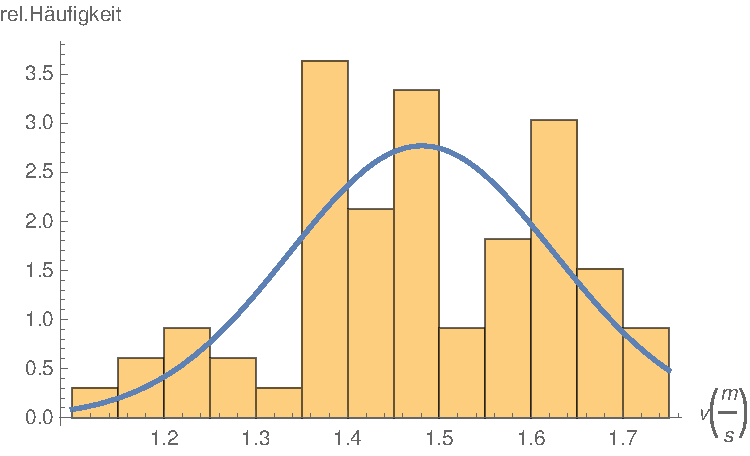
\includegraphics[width=0.8\textwidth]{abbildungen/Histogramm_2017_Ebene.pdf}
\caption{Histogramm der Geschwindigkeiten in der Ebene im Vergleich zur Normalverteilung}
\label{fig:histogramm_ebene}
\end{figure}

Abbildung \ref{fig:qqplot_ebene} veranschaulicht die Verteilung der Geschwindigkeiten in einem Quantil-Quantil Diagramm. In diesem Diagramm sind die gemessenen Geschwindigkeiten gegenüber der Normalverteilung abgebildet. Da sich die Mehrheit der geplotteten Punkte auf oder in unmittelbarer Nähe der Diagonalen befindet, spricht dieses Diagramm für eine Normalverteilung der Geschwindigkeiten. Für eine aussagekräftigere Beurteilung wird diese Thematik im Folgenden mit rechnerischen Tests überprüft.
\begin{figure}[htpb]
\centering
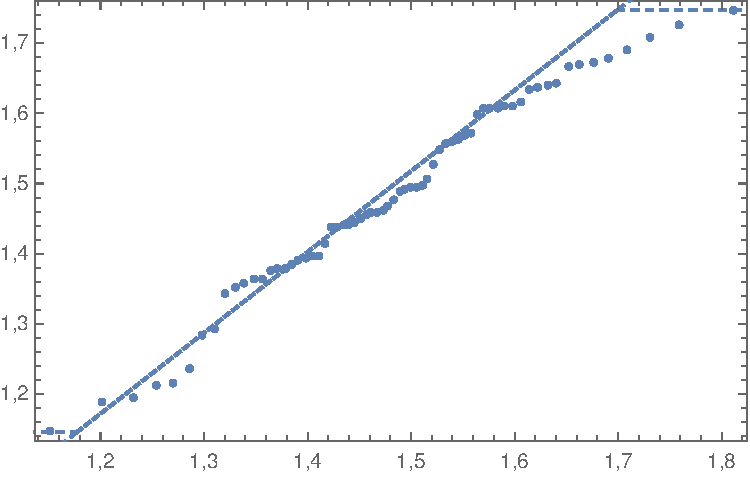
\includegraphics[width=0.7\textwidth]{abbildungen/QQ_Plot_2017_Ebene.pdf}
\caption{Quantil-Quantil-Diagramm der Geschwindigkeiten in der Ebene in $\frac{m}{s}$}
\label{fig:qqplot_ebene}
\end{figure}

\subsubsection{Rechnerische Überprüfung}

Tabelle \ref{tab:anpassungstest_ebene} zeigt die Ergebnisse von mehreren Anpassungstests. Dabei werden die Messdaten auf Normalverteilung getestet. Exemplarisch werden im Folgenden Shapiro-Wilk-, Cramér-von-Mises- und Anderson-Darling-Test näher betrachtet und analysiert.  

Laut dem Shapiro-Wilk-Test wird die Nullhypothese "Die Geschwindigkeiten sind normalverteilt" nicht verworfen, da der P-Wert das Signifikanzniveau von $0,05$ überschreitet. Auch der Cramér-von-Mises-Test ergibt einen P-Wert von $0,84$ und ist somit ebenfalls deutlich über dem Signifikanzniveau. Analog hierzu liefert der Anderson-Darling-Test einen weiteren Nachweis für die Normalverteilung der Geschwindigkeiten, da der P-Wert von $0,82$ die $0,05$ des Signifikanzniveaus ebenfalls überschreitet. (Der Anderson-Darling-Test gilt als aussagekräftigster statistischer Test)

Betrachtet man abschließend alle ermittelten Ergebnisse, kann man davon ausgehen, dass die Geschwindigkeiten der Probanden in der Ebene normalverteilt sind. 
\begin{table}
\centering
\begin{tabular}{l|ll}
 \text{} & \text{Statistic} & \text{P-Value} \\
\hline
 \text{Anderson-Darling} & 0.426988 & 0.821001 \\
 \text{Baringhaus-Henze} & 0.269634 & 0.785711 \\
 \text{Cram{\' e}r-von Mises} & 0.0560719 & 0.838694 \\
 \text{Jarque-Bera ALM} & 1.57313 & 0.376383 \\
 \text{Mardia Combined} & 1.57313 & 0.376383 \\
 \text{Mardia Kurtosis} & -0.879486 & 0.379138 \\
 \text{Mardia Skewness} & 0.82605 & 0.363417 \\
 \text{Pearson }$\chi ^2$ & 14.6667 & 0.144695 \\
 \text{Shapiro-Wilk} & 0.975506 & 0.215767 \\
\end{tabular}
\caption{Anpassungstests zur Überprüfung der gemessenen Geschwindigkeiten in der Ebene auf Normalverteilung}
\label{tab:anpassungstest_ebene}
\end{table}



\subsection{Beim Treppenaufstieg}
\subsubsection{Grafische Überprüfung}
Bei der Betrachtung der Messergebnisse für den Treppenaufstieg fällt auf, dass vier Probanden stets mit höherer Geschwindigkeit gehen als die restlichen Probanden. Dieses Verhalten wiederholt sich über alle Runden. Aufgrund der geringen Anzahl an Messwerten fällt dies bei der Auswertung stark ins Gewicht. 

Für die weitere Überprüfung auf Normalverteilung werden zwei Auswertungen durchgeführt. Eine Auswertung erfolgt über alle Messreihen hinweg. Die betroffenen Probanden haben beim Aufstieg immer mehrere Treppen übersprungen. Es ist nicht auszuschließen, dass es in der Bevölkerung einen Anteil von Menschen gibt, die dieses Verhalten grundsätzlich aufweisen. Anschließend wird eine Auswertung durchgeführt, bei welcher die Ausreißer ausgeschlossen werden, da die Möglichkeit besteht, dass es sich um eine Anomalie oder um Sabotage handelt. 

\begin{figure}[!htb]
    \centering
    \begin{minipage}{.5\textwidth}
        \centering
        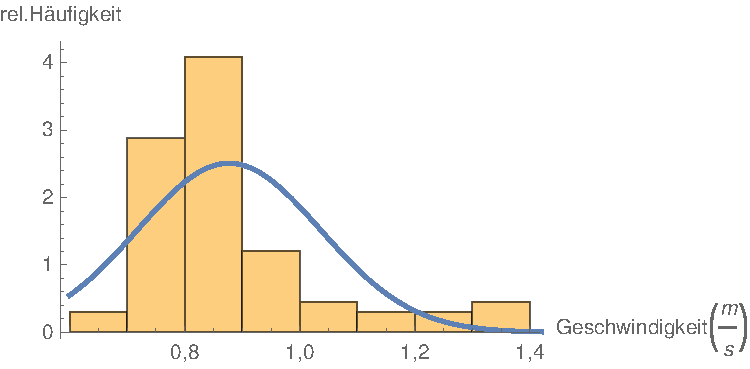
\includegraphics[width=\textwidth]{abbildungen/Histogramm_2017_TreppeAuf_MitAusreisser.pdf}
        \caption{Histogramm der Geschwindig-keiten beim Treppenaufstieg mit Ausreißern im Vergleich zur Normalverteilung}
        \label{fig:Histogramm_TreppeAuf_MA}
    \end{minipage}%
    \begin{minipage}{0.5\textwidth}
        \centering
        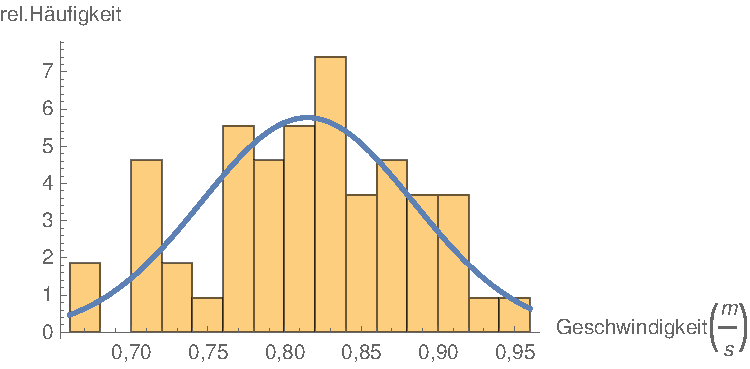
\includegraphics[width=\textwidth]{abbildungen/Histogramm_2017_TreppeAuf_OhneAusreisser.pdf}
        \caption{Histogramm der Geschwindig-keiten beim Treppenaufstieg ohne Ausreißer im Vergleich zur Normalverteilung}
        \label{fig:Histogramm_TreppeAuf_OA}
    \end{minipage}
\end{figure}

Das Histogramm in der Abbildung \ref{fig:Histogramm_TreppeAuf_MA} deutet auf eine rechtsschiefe Verteilung der Geschwindigkeiten hin. Dies stellt ein Indiz gegen eine Normalverteilung der Messwerte dar. Im Gegensatz dazu weist das Histogramm in Abbildung \ref{fig:Histogramm_TreppeAuf_OA} eine symmetrische Verteilung auf. Daher ist anzunehmen, dass die Messwerte ohne Ausreißer normalverteilt sind. Aber wie bereits erwähnt, sind Histogramme nur bedingt aussagekräftig. Eine genauere grafische Betrachtung erfolgt über ein Quantil-Quantil-Diagramm.

In Abbildung \ref{fig:QQ_TreppeAuf_MA} ist deutlich eine Abweichung von der Normalverteilung zu sehen, da einige Werte weit von der Diagonalen entfernt sind. Dies ist auf die erwähnten vier Probanden zurückzuführen. Im Gegensatz dazu deutet die Abbildung \ref{fig:QQ_TreppeAuf_OA} auf eine Normalverteilung hin, da alle Quantile auf oder in unmittelbarer Nähe der Diagonalen liegen.
\begin{figure}[!htb]
    \centering
    \begin{minipage}{.5\textwidth}
        \centering
        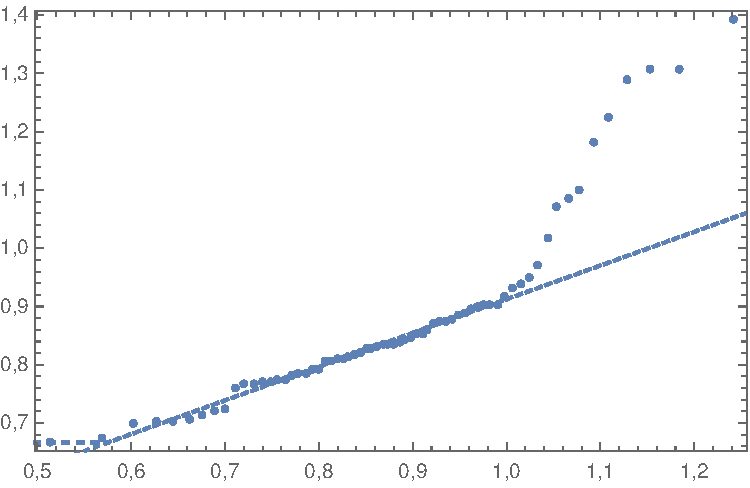
\includegraphics[width=\textwidth]{abbildungen/QQ_Plot_2017_TreppeAuf_MitAusreisser.pdf}
        \caption{Quantil-Quantil-Diagramm der Geschwindigkeiten beim Treppenaufstieg mit Ausreißern in $\frac{m}{s}$}
        \label{fig:QQ_TreppeAuf_MA}
    \end{minipage}%
    \begin{minipage}{0.5\textwidth}
        \centering
        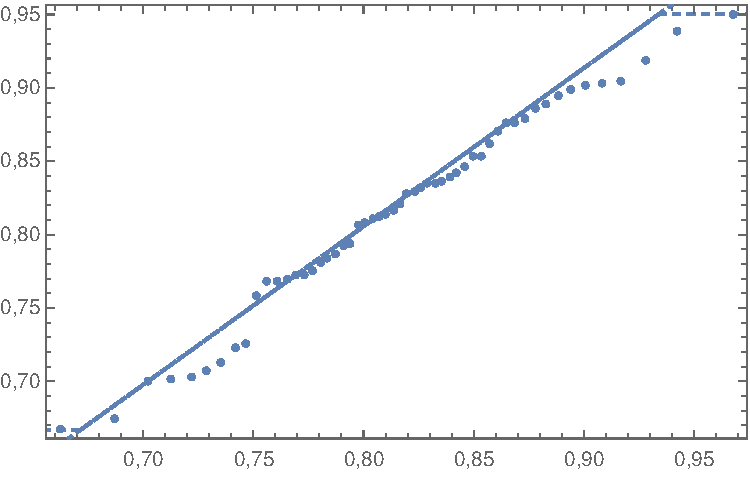
\includegraphics[width=\textwidth]{abbildungen/QQ_Plot_2017_TreppeAuf_OhneAusreisser.pdf}
        \caption{Quantil-Quantil-Diagramm der Geschwindigkeiten beim Treppenaufstieg ohne Ausreißer in $\frac{m}{s}$}
        \label{fig:QQ_TreppeAuf_OA}
    \end{minipage}
\end{figure}


\subsubsection{Rechnerische Überprüfung}
Die Anpassungstests zeigen, dass die Geschwindigkeiten bei einem Treppenaufstieg nicht normalverteilt sind, wenn man die Ausreißer mitberücksichtigt. Die Tabelle \ref{tab:anpassungstest_TreppeAuf_MA} zeigt, dass bei einem Cram{\' e}r-von Mises Test ein p-Wert von nur $0,018$ erreicht wird, welcher somit deutlich geringer als das Signifikanzniveau von $0,05$ ist. Werden die Ausreißer nicht mitberücksichtigt, so ergibt der Cram{\' e}r-von Mises Test einen p-Wert von $0,92$, wie in Tabelle \ref{tab:anpassungstest_TreppeAuf_OA} zu sehen. Auch der Anderson-Darling Test liegt weit über dem Signifikanzniveau. Die rechnerische Überprüfung bestätigt somit das Ergebnis der grafischen Analyse. Wie bereits erwähnt, sind die Ausreißer immer von denselben vier Probanden verursacht worden. Diese haben beim Aufsteigen der Treppen in jeder Runde mehrere Stufen übersprungen. Die Vermutung liegt nahe, dass es eine Gruppe von Menschen gibt, die beim Aufsteigen der Treppen grundsätzlich schneller gehen. Eine genaue Untersuchung ist mit einer deutlich größeren Anzahl der Probanden notwendig.
\begin{table}
    \centering
    \begin{minipage}{.47\textwidth}
\centering
\begin{tabular}{l|ll}
 \text{} & \text{Statistic} & \text{P-Value} \\
\hline
 \text{Anderson-Darling} & 0.33829 & 0.90645 \\
 \text{Baringhaus-Henze} & 0.213705 & 0.858651 \\
 \text{Cram{\' e}r-von Mises} & 0.0421682 & 0.921661 \\
 \text{Jarque-Bera ALM} & 1.31475 & 0.440072 \\
 \text{Mardia Combined} & 1.31475 & 0.440072 \\
 \text{Mardia Kurtosis} & -0.891517 & 0.372652 \\
 \text{Mardia Skewness} & 0.553342 & 0.456956 \\
 \text{Pearson }$\chi ^2$ & 12.2963 & 0.197116 \\
 \text{Shapiro-Wilk} & 0.977864 & 0.414303 \\
\end{tabular}
\caption{Anpassungstests zur Überprüfung der gemessenen Geschwindigkeiten beim Treppenaufstieg ohne Ausreissern auf Normalverteilung}
\label{tab:anpassungstest_TreppeAuf_OA}
    \end{minipage}%
    \begin{minipage}{0.06\textwidth}
     \hfill
    \end{minipage}%
    \begin{minipage}{0.47\textwidth}
\centering
\begin{tabular}{l|ll}
 \text{} & \text{Statistic} & \text{P-Value} \\
\hline
 \text{Anderson-Darling} & 3.67396 & 0.0126832 \\
 \text{Baringhaus-Henze} & 4.53865 & 0.000403182 \\
 \text{Cram{\' e}r-von Mises} & 0.638786 & 0.0179638 \\
 \text{Jarque-Bera ALM} & 45.2212 & 0.000864057 \\
 \text{Mardia Combined} & 45.2212 & 0.000864057 \\
 \text{Mardia Kurtosis} & 3.44345 & 0.000574336 \\
 \text{Mardia Skewness} & 26.5574 & \text{2.55817*$10^{-7}$} \\
 \text{Pearson }$\chi ^2$ & 25. & 0.00534551 \\
 \text{Shapiro-Wilk} & 0.835009 & \text{4.31299*$10^{-7}$} \\
\end{tabular}
\caption{Anpassungstests zur Überprüfung der gemessenen Geschwindigkeiten beim Treppenaufstieg mit Ausreissern auf Normalverteilung}
\label{tab:anpassungstest_TreppeAuf_MA}
    \end{minipage}
\end{table}

\subsection{Beim Treppenabstieg}

Bei der Messung zum Abstieg von der Treppe gibt es wenig besondere Fälle. Die gemessenen Daten weisen nur wenige unregelmäßige Ausreißer aus. Diese werden erwartungsgemäß geringen Einfluss haben. Beim Treppenaufstieg wurden signifikante Unterschiede durch 
die Ausreißer festgestellt. Deswegen werden analog zum Aufstieg beim Abstieg auch zwei Analysen durchgeführt.



\subsubsection{Grafische Überprüfung}
Ein Vergleich der Histogramme in den Abbildungen \ref{fig:Histogramm_TreppeAb_MA} und \ref{fig:Histogramm_TreppeAb_OA} zeigt, dass die Ausreißer nur einen geringen Unterschied verursachen. In den Abbildungen ist jeweils eine Normalverteilungskurve dargestellt. Es zeigt sich, dass eine Normalverteilung nicht genau erkennbar ist.

Beim Betrachten des Quantil-Quantil-Diagramms in Abbildung \ref{fig:QQ_TreppeAb_MA} und \ref{fig:QQ_TreppeAb_OA}, zeigt sich ebenfalls, dass der Unterschied der gesamten Daten und der bereinigten Daten sehr gering und mit bloßem Auge nicht zu erkennen ist. Aus den beiden Diagrammen wird deutlich, dass es sich bei beiden Fällen um eine Normalverteilung handelt, da der P-Wert in beiden Fällen über dem Signifikanzniveau von $0,05$ liegt.

\begin{figure}[!htb]
    \centering
    \begin{minipage}{.49\textwidth}
        \centering
        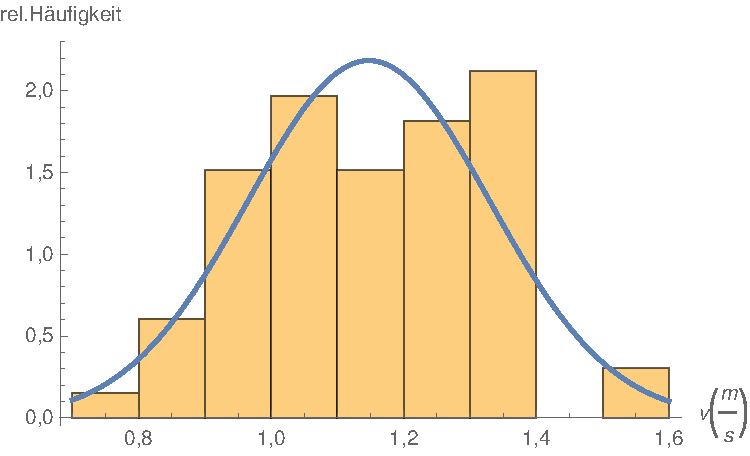
\includegraphics[width=\textwidth]{abbildungen/Histogramm_2017_TreppeAb_MitAusreisser.pdf}
        \caption{Histogramm der Geschwindig-keiten beim Treppenabstieg mit Ausreißern im Vergleich zur Normalverteilung}
        \label{fig:Histogramm_TreppeAb_MA}
    \end{minipage}%
    \begin{minipage}{0.02\textwidth}
     \hfill
    \end{minipage}%
    \begin{minipage}{0.49\textwidth}
        \centering
        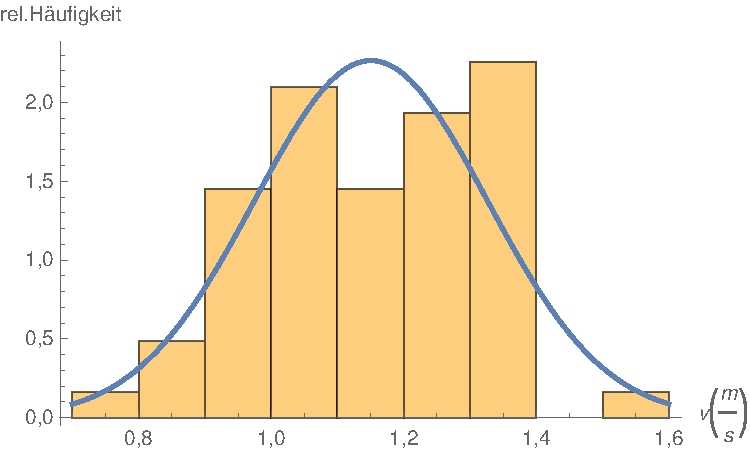
\includegraphics[width=\textwidth]{abbildungen/Histogramm_2017_TreppeAb_OhneAusreisser.pdf}
        \caption{Histogramm der Geschwindig-keiten beim Treppenabstieg ohne Ausreißer im Vergleich zur Normalverteilung}
        \label{fig:Histogramm_TreppeAb_OA}
    \end{minipage}
\end{figure}


\begin{figure}[!htb]
    \centering
    \begin{minipage}{.49\textwidth}
        \centering
        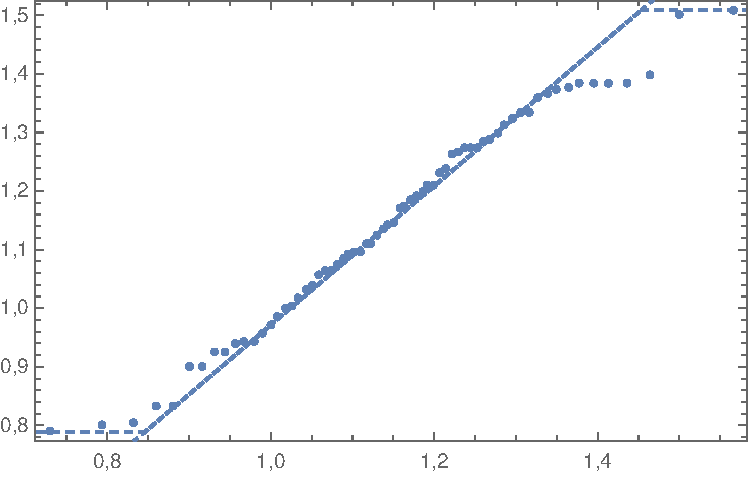
\includegraphics[width=\textwidth]{abbildungen/QQ_Plot_2017_TreppeAb_MitAusreisser.pdf}
        \caption{Quantil-Quantil-Diagramm der Geschwindigkeiten beim Treppenabstieg mit Ausreißern in $\frac{m}{s}$}
        \label{fig:QQ_TreppeAb_MA}
    \end{minipage}%
    \begin{minipage}{0.02\textwidth}
     \hfill
    \end{minipage}%
    \begin{minipage}{0.49\textwidth}
        \centering
        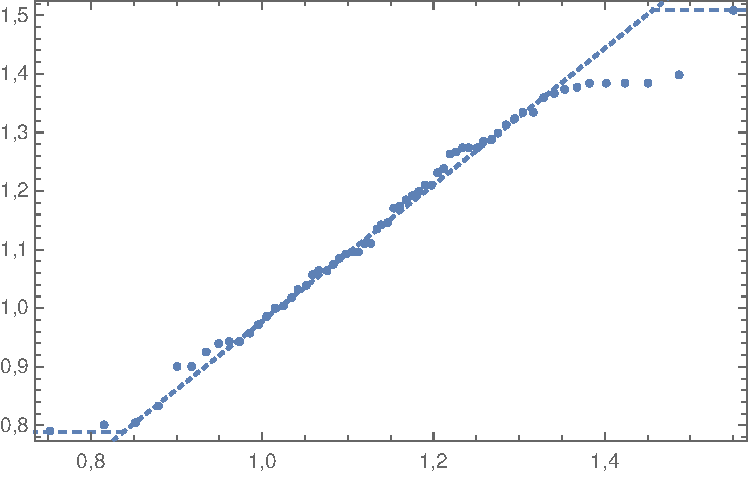
\includegraphics[width=\textwidth]{abbildungen/QQ_Plot_2017_TreppeAb_OhneAusreisser.pdf}
        \caption{Quantil-Quantil-Diagramm der Geschwindigkeiten beim Treppenabstieg ohne Ausreißer in $\frac{m}{s}$}
        \label{fig:QQ_TreppeAb_OA}
    \end{minipage}
\end{figure}




\subsection{Rechnerische Überprüfung}
Die rechnerische Überprüfung bestätigt die Analyse des Quantil-Quantil-Diagramms. Wie in Tabelle \ref{tab:anpassungstest_TreppeAb_MA} und Tabelle \ref{tab:anpassungstest_TreppeAbf_OA} zu sehen, liegt in beiden Fällen eine Normalverteilung vor. Es ist zu bemerken, dass ein Anpassungstest anhand der Daten mit Ausreißern einen größeren p-Wert erzielt. 
\begin{table}
    \centering
    \begin{minipage}{.47\textwidth}
\centering
\begin{tabular}{l|ll}
  \text{} & \text{Statistic} & \text{P-Value} \\
\hline
 \text{Anderson-Darling} & 0.440903 & 0.806782 \\
 \text{Baringhaus-Henze} & 0.420106 & 0.556077 \\
 \text{Cram{\' e}r-von Mises} & 0.0609776 & 0.807822 \\
 \text{Jarque-Bera ALM} & 2.23559 & 0.247476 \\
 \text{Mardia Combined} & 2.23559 & 0.247476 \\
 \text{Mardia Kurtosis} & -1.43247 & 0.152009 \\
 \text{Mardia Skewness} & 0.156589 & 0.692316 \\
 \text{Pearson }$\chi ^2$ & 10.3333 & 0.411752 \\
 \text{Shapiro-Wilk} & 0.974316 & 0.186898 \\
\end{tabular}
\caption{Anpassungstests zur Überprüfung der gemessenen Geschwindigkeiten beim Treppenabstieg mit Ausreissern auf Normalverteilung}
\label{tab:anpassungstest_TreppeAb_MA}
    \end{minipage}%
    \begin{minipage}{0.06\textwidth}
     \hfill
    \end{minipage}%
    \begin{minipage}{0.47\textwidth}
\centering
\begin{tabular}{l|ll}
 \text{} & \text{Statistic} & \text{P-Value} \\
\hline
 \text{Anderson-Darling} & 0.54237 & 0.70308 \\
 \text{Baringhaus-Henze} & 0.484286 & 0.455989 \\
 \text{Cram{\' e}r-von Mises} & 0.0788816 & 0.698349 \\
 \text{Jarque-Bera ALM} & 1.99557 & 0.277317 \\
 \text{Mardia Combined} & 1.99557 & 0.277317 \\
 \text{Mardia Kurtosis} & -1.32774 & 0.184265 \\
 \text{Mardia Skewness} & 0.190686 & 0.662346 \\
 \text{Pearson }$\chi ^2$ & 6.37037 & 0.702354 \\
 \text{Shapiro-Wilk} & 0.969539 & 0.183952 \\
\end{tabular}
\caption{Anpassungstests zur Überprüfung der gemessenen Geschwindigkeiten beim Treppenabstieg ohne Ausreissern auf Normalverteilung}
\label{tab:anpassungstest_TreppeAbf_OA}
    \end{minipage}
\end{table}

\section{Modell}
\section{Lineare Regression}
\subsection{Prüfung auf eine Abhängigkeit}
\subsection{Mehrere Abhängigkeiten}
\subsection{Konditionierung}
Die Konditionierung des Problems wurde anhand der Desingmatrix des linearen Modells untersucht. Je näher ein ermittelter Wert an 1 liegt, desto besser ist das Problem konditioniert.

Bei der Untersuchung der Treppengeschwindigkeit aufwärts wurde ein Konditionierungswert von $744.683$ ermittelt. Auch bei der Betrachtung der Treppengeschwindigkeit abwärts wurde ähnliches Ergebnis von $654.274$ berechnet. Die Betrachtung zweier Parameter (Ebenengeschwindigkeit und Körpergröße) ergab sogar den Wert $3.27621*10^7$.
Diese schlechte Konditionierung erfolgt durch Rechenfehlern, die bei numerischen Berechnungen erfolgen. In diesen Berechnungen wurden 3 ($2.87197$, $2.81576$) bzw. $7.47687$ Dezimalstellen verloren. Diese Zahlen wurden mit wurden mit dem dekadischen Logarithmus (zur Basis 10) der Kondition bestimmt.

Wenn man die Konditionierung mit der QR-Zerlegung betrachtet, welche auch in Wirklichkeit von Mathematica verwendet wird, wurde eine wesentlich bessere Konditionierung ermittelt.

Die Betrachtung der Konditionierung der oberen Dreiecksmatrix R ergab bei der Treppengeschwindigkeit aufwärts nun einen Wert von $29.6338$. Hierbei wurden auch weniger verlorene Dezimalstellen festgestellt. Diese betrugen nur noch $1.47179$. Bei der Treppengeschwindigkeit abwärts wurde eine Konditionierung von $27.9171$ und $7164.48$ bei zwei Parametern (Verlorene Dezimalstellen bei $1.44587$ bzw. $3.83839$). Bei einem Parameter - der Ebenengeschwindigkeit - ist die Konditionierung nun deutlich besser. Für zwei Parameter (Körpergröße und Ebenengeschwindigkeit) lässt sich schließen, dass für diese Auswertung das Problem tatsächlich schlecht Konditioniert ist und die Aussagekraft der Ergebnisse bei dieser Untersuchung in Frage gestellt werden kann.

Dadurch, dass Mathematica die QR-Zerlegung benutzt sind diese Ergebnisse auch wesentlich aussagekräftiger als die erste Untersuchung der Konditionierung.



\section{Ergebnisse}
\section{Ermitteltes Modell}

\section{Vergleich mit Daten aus 2012}
\subsection{Überprüfung auf Normalverteilung}
\subsection{Lineare Regression}
\subsection{Vergleich}

\section{Verbund von alten und neuen Daten}

\section{Fazit}
In dieser Arbeit ging es darum einen möglichen Zusammenhang zwischen der Wunschgeschwindigkeit einer Person auf der Ebene und den Geschwindigkeiten auf einer Treppe zu untersuchen. Dabei wurde das Laufverhalten sowohl aufwärts als auch abwärts betrachtet. Es wurden Messreihen durchgeführt, bei denen Probanden mit Stoppuhren deren Dauer gemessen haben, die sie benötigt haben um definierte Strecken abzulaufen. Die gewonnenen Daten wurden daraufhin auf Normalverteilung untersucht. Anschließend wurde die lineare Regression verwendet um mögliche Verbindungen zwischen den Treppengeschwindigkeiten und den Parametern der Probanden, wie Ebenengeschwindigkeit, Körpergröße oder die Rundennummer zu erkennen. Mithilfe der t-Tests wurden die resultierenden Werte auf Plausibilität geprüft. Dabei wurde entschieden ob es Abhängigkeiten gibt. Zur Überprüfung der Relevanz dieser Beobachtungen wurde die Konditionierung des Problems untersucht. Die gewonnenen Erkenntnisse wurden mit Messdaten aus einem bereits im Jahr 2012 durchgeführten Experiments verglichen und verbunden.

Die Resultate dieser Arbeit können keine 100\%tige Bestimmung des Laufverhaltens eines Menschen auf einer Treppe durch die Wunschgeschwindigkeit auf der Ebene bieten. Für solch ein Wissen ist das Laufverhalten von Personen noch nicht ausreichend untersucht. Für noch genauere Ergebnisse und Vorhersagen würden sich zukünftige Messreihen mit wesentlich mehr als $22$ Probanden anbieten. 

\end{document}
